\chapter{$F$-symbols for the $\mathcal{H}_3$ fusion category}
\label{app:Fsymbols}

This solution and the code which was used to calculate it can be found under \url{https://github.com/R8monaW/H3Fsymbols}. It is a real solution with two parameters, $p_1,p_2\in\{-1,+1\}$. Additionally, we use the following notation:
	\begin{align}
		A&=\frac{1}{2} \left(\sqrt{13}-3\right),\\
		B&=\frac{1}{3} \left(\sqrt{13}-2\right),\\
		C&=\frac{1}{6} \left(\sqrt{13}+1\right),\\
		D_{\pm}&=\frac{1}{12} \left(5-\sqrt{13}\pm\sqrt{6 \left(\sqrt{13}+1\right)}\right).
	\end{align}
In the following, all $F$-symbols are listed. They are first ordered by their dimension and within that, they are ordered by their labels. The $3$- and $4$-dimensional matrices are depicted as tables where the first row and the first column indicate the admissible labels for the matrix.

Since all occurring values of the $F$-symbols are in the interval $[-1,+1]$, we can visualise this solution as follows: We represent the value $+1$ with a black pixel and the value $-1$ with a white pixel. The values in between are depicted by a green pixel whose darkness depends on where the value lies in the interval $[-1,+1]$, e.g., a value close to $+1$ is depicted by a very dark green pixel, while a value close to $-1$ is depicted by a very light green pixel. For parameter values $p_1=p_2=+1$, this is shown in \cref{fig:pixels}, where the order of the $F$-symbols is chosen randomly.

\begin{figure}[H]
	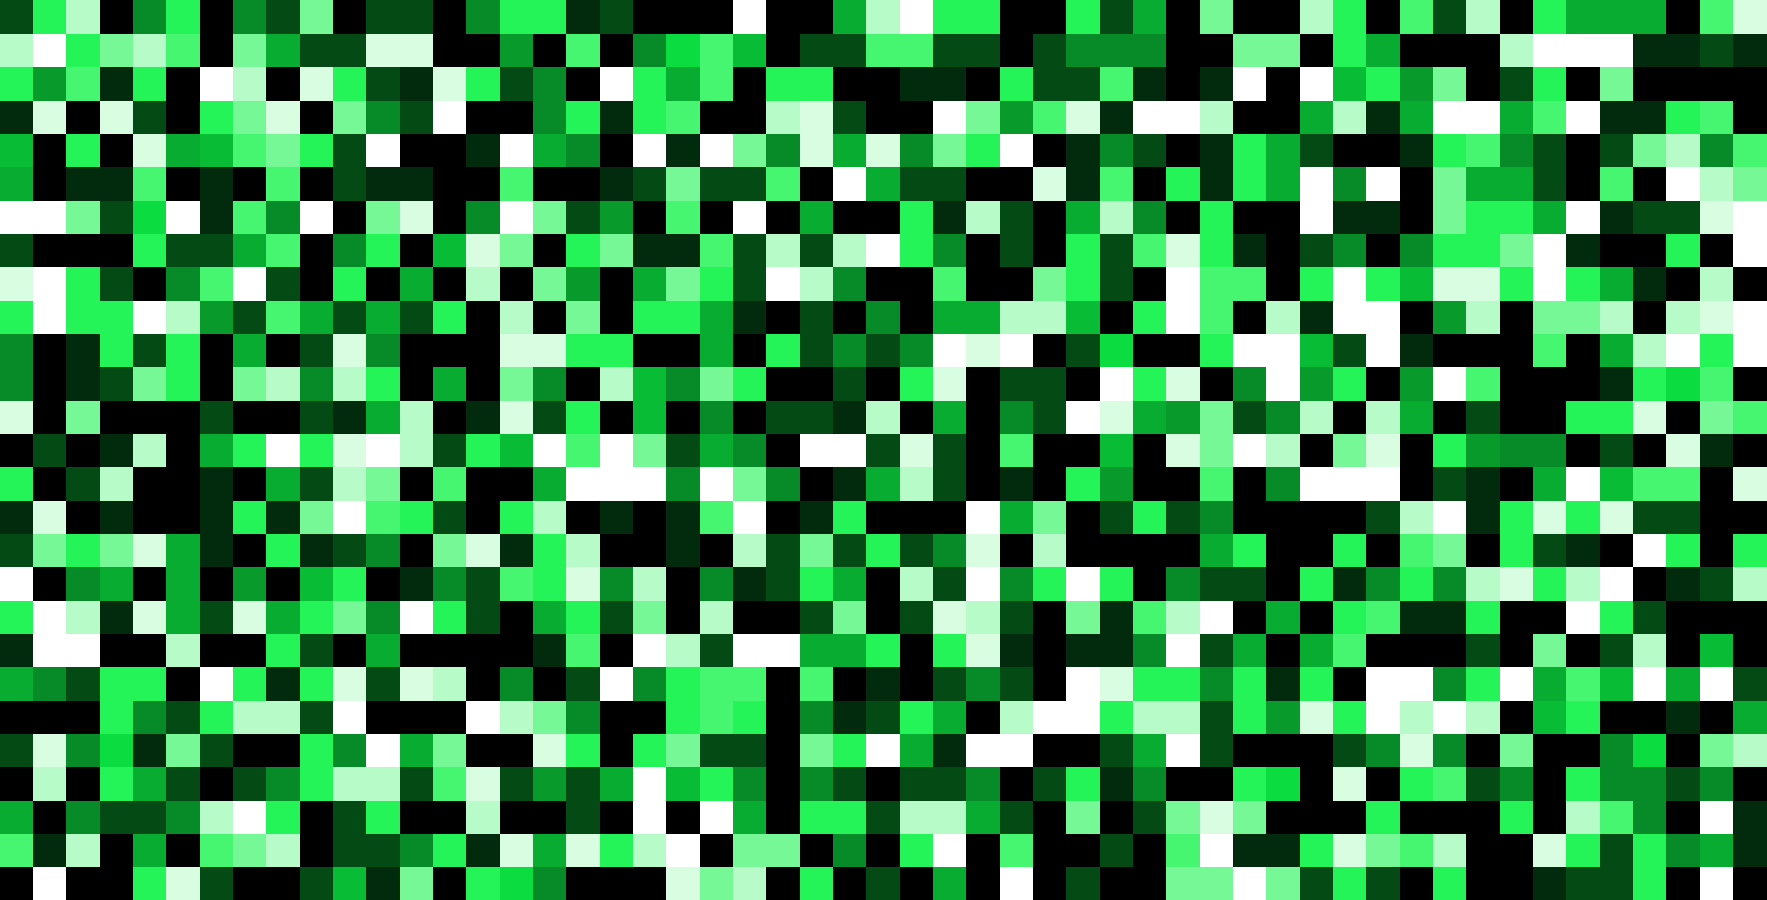
\includegraphics[width=0.65\textwidth]{solution_pic.pdf}
	\caption{\small \textbf{A visualisation of the $F$-symbols.} To generate this picture, we set the parameters to $p_1=p_2=+1$ and choose a random ordering of the $F$-symbols.}
	\label{fig:pixels}
\end{figure}

\section{$1$-dimensional $F$-symbols}
{\allowdisplaybreaks\begin{align}
F_{1}^{111}&=1&F_{1}^{1\alpha\alpha^*}&=1&F_{1}^{1\alpha^*\alpha}&=1&F_{1}^{1\rho\rho}&=1\\F_{1}^{1{}_\alpha\rho{}_\alpha\rho}&=1&F_{1}^{1\alphastarrho\alphastarrho}&=1&F_{1}^{\alpha1\alpha^*}&=1&F_{1}^{\alpha\alpha\alpha}&=1\\F_{1}^{\alpha\alpha^*1}&=1&F_{1}^{\alpha\rho{}_\alpha\rho}&=1&F_{1}^{\alpha{}_\alpha\rho\alphastarrho}&=-p_1&F_{1}^{\alpha\alphastarrho\rho}&=1\\F_{1}^{\alpha^*1\alpha}&=1&F_{1}^{\alpha^*\alpha1}&=1&F_{1}^{\alpha^*\alpha^*\alpha^*}&=1&F_{1}^{\alpha^*\rho\alphastarrho}&=1\\F_{1}^{\alpha^*{}_\alpha\rho\rho}&=1&F_{1}^{\alpha^*\alphastarrho{}_\alpha\rho}&=-p_1&F_{1}^{\rho1\rho}&=1&F_{1}^{\rho\alpha\alphastarrho}&=1\\F_{1}^{\rho\alpha^*{}_\alpha\rho}&=1&F_{1}^{\rho\rho1}&=1&F_{1}^{\rho\rho\rho}&=1&F_{1}^{\rho\rho{}_\alpha\rho}&=1\\F_{1}^{\rho\rho\alphastarrho}&=1&F_{1}^{\rho{}_\alpha\rho\alpha}&=1&F_{1}^{\rho{}_\alpha\rho\rho}&=1&F_{1}^{\rho{}_\alpha\rho{}_\alpha\rho}&=1\\F_{1}^{\rho{}_\alpha\rho\alphastarrho}&=-1&F_{1}^{\rho\alphastarrho\alpha^*}&=1&F_{1}^{\rho\alphastarrho\rho}&=1&F_{1}^{\rho\alphastarrho{}_\alpha\rho}&=p_1p_2\\F_{1}^{\rho\alphastarrho\alphastarrho}&=-p_1p_2&F_{1}^{{}_\alpha\rho1{}_\alpha\rho}&=1&F_{1}^{{}_\alpha\rho\alpha\rho}&=1&F_{1}^{{}_\alpha\rho\alpha^*\alphastarrho}&=1\\F_{1}^{{}_\alpha\rho\rho\alpha^*}&=1&F_{1}^{{}_\alpha\rho\rho\rho}&=1&F_{1}^{{}_\alpha\rho\rho{}_\alpha\rho}&=1&F_{1}^{{}_\alpha\rho\rho\alphastarrho}&=p_2\\F_{1}^{{}_\alpha\rho{}_\alpha\rho1}&=1&F_{1}^{{}_\alpha\rho{}_\alpha\rho\rho}&=1&F_{1}^{{}_\alpha\rho{}_\alpha\rho{}_\alpha\rho}&=1&F_{1}^{{}_\alpha\rho{}_\alpha\rho\alphastarrho}&=-1\\F_{1}^{{}_\alpha\rho\alphastarrho\alpha}&=-p_1&F_{1}^{{}_\alpha\rho\alphastarrho\rho}&=p_1&F_{1}^{{}_\alpha\rho\alphastarrho{}_\alpha\rho}&=1&F_{1}^{{}_\alpha\rho\alphastarrho\alphastarrho}&=-1\\F_{1}^{\alphastarrho1\alphastarrho}&=1&F_{1}^{\alphastarrho\alpha{}_\alpha\rho}&=1&F_{1}^{\alphastarrho\alpha^*\rho}&=1&F_{1}^{\alphastarrho\rho\alpha}&=1\\F_{1}^{\alphastarrho\rho\rho}&=1&F_{1}^{\alphastarrho\rho{}_\alpha\rho}&=-p_1&F_{1}^{\alphastarrho\rho\alphastarrho}&=1&F_{1}^{\alphastarrho{}_\alpha\rho\alpha^*}&=-p_1\\F_{1}^{\alphastarrho{}_\alpha\rho\rho}&=p_1&F_{1}^{\alphastarrho{}_\alpha\rho{}_\alpha\rho}&=-1&F_{1}^{\alphastarrho{}_\alpha\rho\alphastarrho}&=1&F_{1}^{\alphastarrho\alphastarrho1}&=1\\F_{1}^{\alphastarrho\alphastarrho\rho}&=-p_1p_2&F_{1}^{\alphastarrho\alphastarrho{}_\alpha\rho}&=-1&F_{1}^{\alphastarrho\alphastarrho\alphastarrho}&=1&F_{\alpha}^{11\alpha}&=1\\F_{\alpha}^{1\alpha1}&=1&F_{\alpha}^{1\alpha^*\alpha^*}&=1&F_{\alpha}^{1\rho\alphastarrho}&=1&F_{\alpha}^{1{}_\alpha\rho\rho}&=1\\F_{\alpha}^{1\alphastarrho{}_\alpha\rho}&=1&F_{\alpha}^{\alpha11}&=1&F_{\alpha}^{\alpha\alpha\alpha^*}&=1&F_{\alpha}^{\alpha\alpha^*\alpha}&=1\\F_{\alpha}^{\alpha\rho\rho}&=1&F_{\alpha}^{\alpha{}_\alpha\rho{}_\alpha\rho}&=1&F_{\alpha}^{\alpha\alphastarrho\alphastarrho}&=1&F_{\alpha}^{\alpha^*1\alpha^*}&=1\\F_{\alpha}^{\alpha^*\alpha\alpha}&=1&F_{\alpha}^{\alpha^*\alpha^*1}&=1&F_{\alpha}^{\alpha^*\rho{}_\alpha\rho}&=1&F_{\alpha}^{\alpha^*{}_\alpha\rho\alphastarrho}&=-p_1\\F_{\alpha}^{\alpha^*\alphastarrho\rho}&=-p_1&F_{\alpha}^{\rho1\alphastarrho}&=1&F_{\alpha}^{\rho\alpha{}_\alpha\rho}&=-p_1&F_{\alpha}^{\rho\alpha^*\rho}&=-1\\F_{\alpha}^{\rho\rho\alpha}&=1&F_{\alpha}^{\rho\rho\rho}&=1&F_{\alpha}^{\rho\rho{}_\alpha\rho}&=1&F_{\alpha}^{\rho\rho\alphastarrho}&=1\\F_{\alpha}^{\rho{}_\alpha\rho\alpha^*}&=-p_1&F_{\alpha}^{\rho{}_\alpha\rho\rho}&=p_1&F_{\alpha}^{\rho{}_\alpha\rho{}_\alpha\rho}&=p_1&F_{\alpha}^{\rho{}_\alpha\rho\alphastarrho}&=1\\F_{\alpha}^{\rho\alphastarrho1}&=1&F_{\alpha}^{\rho\alphastarrho\rho}&=-p_1p_2&F_{\alpha}^{\rho\alphastarrho{}_\alpha\rho}&=p_1&F_{\alpha}^{\rho\alphastarrho\alphastarrho}&=1\\F_{\alpha}^{{}_\alpha\rho1\rho}&=1&F_{\alpha}^{{}_\alpha\rho\alpha\alphastarrho}&=-1&F_{\alpha}^{{}_\alpha\rho\alpha^*{}_\alpha\rho}&=-1&F_{\alpha}^{{}_\alpha\rho\rho1}&=1\\F_{\alpha}^{{}_\alpha\rho\rho\rho}&=1&F_{\alpha}^{{}_\alpha\rho\rho{}_\alpha\rho}&=1&F_{\alpha}^{{}_\alpha\rho\rho\alphastarrho}&=-1&F_{\alpha}^{{}_\alpha\rho{}_\alpha\rho\alpha}&=1\\F_{\alpha}^{{}_\alpha\rho{}_\alpha\rho\rho}&=1&F_{\alpha}^{{}_\alpha\rho{}_\alpha\rho{}_\alpha\rho}&=1&F_{\alpha}^{{}_\alpha\rho{}_\alpha\rho\alphastarrho}&=-1&F_{\alpha}^{{}_\alpha\rho\alphastarrho\alpha^*}&=-p_1\\F_{\alpha}^{{}_\alpha\rho\alphastarrho\rho}&=1&F_{\alpha}^{{}_\alpha\rho\alphastarrho{}_\alpha\rho}&=1&F_{\alpha}^{{}_\alpha\rho\alphastarrho\alphastarrho}&=-p_1p_2&F_{\alpha}^{\alphastarrho1{}_\alpha\rho}&=1\\F_{\alpha}^{\alphastarrho\alpha\rho}&=p_1&F_{\alpha}^{\alphastarrho\alpha^*\alphastarrho}&=1&F_{\alpha}^{\alphastarrho\rho\alpha^*}&=1&F_{\alpha}^{\alphastarrho\rho\rho}&=p_1\\F_{\alpha}^{\alphastarrho\rho{}_\alpha\rho}&=1&F_{\alpha}^{\alphastarrho\rho\alphastarrho}&=p_2&F_{\alpha}^{\alphastarrho{}_\alpha\rho1}&=1&F_{\alpha}^{\alphastarrho{}_\alpha\rho\rho}&=-p_1\\F_{\alpha}^{\alphastarrho{}_\alpha\rho{}_\alpha\rho}&=1&F_{\alpha}^{\alphastarrho{}_\alpha\rho\alphastarrho}&=-1&F_{\alpha}^{\alphastarrho\alphastarrho\alpha}&=1&F_{\alpha}^{\alphastarrho\alphastarrho\rho}&=-1\\F_{\alpha}^{\alphastarrho\alphastarrho{}_\alpha\rho}&=1&F_{\alpha}^{\alphastarrho\alphastarrho\alphastarrho}&=-p_1p_2&F_{\alpha^*}^{11\alpha^*}&=1&F_{\alpha^*}^{1\alpha\alpha}&=1\\F_{\alpha^*}^{1\alpha^*1}&=1&F_{\alpha^*}^{1\rho{}_\alpha\rho}&=1&F_{\alpha^*}^{1{}_\alpha\rho\alphastarrho}&=1&F_{\alpha^*}^{1\alphastarrho\rho}&=1\\F_{\alpha^*}^{\alpha1\alpha}&=1&F_{\alpha^*}^{\alpha\alpha1}&=1&F_{\alpha^*}^{\alpha\alpha^*\alpha^*}&=1&F_{\alpha^*}^{\alpha\rho\alphastarrho}&=-p_1\\F_{\alpha^*}^{\alpha{}_\alpha\rho\rho}&=1&F_{\alpha^*}^{\alpha\alphastarrho{}_\alpha\rho}&=1&F_{\alpha^*}^{\alpha^*11}&=1&F_{\alpha^*}^{\alpha^*\alpha\alpha^*}&=1\\F_{\alpha^*}^{\alpha^*\alpha^*\alpha}&=1&F_{\alpha^*}^{\alpha^*\rho\rho}&=1&F_{\alpha^*}^{\alpha^*{}_\alpha\rho{}_\alpha\rho}&=1&F_{\alpha^*}^{\alpha^*\alphastarrho\alphastarrho}&=1\\F_{\alpha^*}^{\rho1{}_\alpha\rho}&=1&F_{\alpha^*}^{\rho\alpha\rho}&=-1&F_{\alpha^*}^{\rho\alpha^*\alphastarrho}&=p_1&F_{\alpha^*}^{\rho\rho\alpha^*}&=1\\F_{\alpha^*}^{\rho\rho\rho}&=-1&F_{\alpha^*}^{\rho\rho{}_\alpha\rho}&=1&F_{\alpha^*}^{\rho\rho\alphastarrho}&=-p_1p_2&F_{\alpha^*}^{\rho{}_\alpha\rho1}&=1\\F_{\alpha^*}^{\rho{}_\alpha\rho\rho}&=1&F_{\alpha^*}^{\rho{}_\alpha\rho{}_\alpha\rho}&=1&F_{\alpha^*}^{\rho{}_\alpha\rho\alphastarrho}&=p_1&F_{\alpha^*}^{\rho\alphastarrho\alpha}&=1\\F_{\alpha^*}^{\rho\alphastarrho\rho}&=p_1&F_{\alpha^*}^{\rho\alphastarrho{}_\alpha\rho}&=1&F_{\alpha^*}^{\rho\alphastarrho\alphastarrho}&=p_2&F_{\alpha^*}^{{}_\alpha\rho1\alphastarrho}&=1\\F_{\alpha^*}^{{}_\alpha\rho\alpha{}_\alpha\rho}&=-1&F_{\alpha^*}^{{}_\alpha\rho\alpha^*\rho}&=-p_1&F_{\alpha^*}^{{}_\alpha\rho\rho\alpha}&=-p_1&F_{\alpha^*}^{{}_\alpha\rho\rho\rho}&=-p_1\\F_{\alpha^*}^{{}_\alpha\rho\rho{}_\alpha\rho}&=p_1&F_{\alpha^*}^{{}_\alpha\rho\rho\alphastarrho}&=1&F_{\alpha^*}^{{}_\alpha\rho{}_\alpha\rho\alpha^*}&=1&F_{\alpha^*}^{{}_\alpha\rho{}_\alpha\rho\rho}&=-1\\F_{\alpha^*}^{{}_\alpha\rho{}_\alpha\rho{}_\alpha\rho}&=-1&F_{\alpha^*}^{{}_\alpha\rho{}_\alpha\rho\alphastarrho}&=1&F_{\alpha^*}^{{}_\alpha\rho\alphastarrho1}&=1&F_{\alpha^*}^{{}_\alpha\rho\alphastarrho\rho}&=p_1\\F_{\alpha^*}^{{}_\alpha\rho\alphastarrho{}_\alpha\rho}&=-1&F_{\alpha^*}^{{}_\alpha\rho\alphastarrho\alphastarrho}&=1&F_{\alpha^*}^{\alphastarrho1\rho}&=1&F_{\alpha^*}^{\alphastarrho\alpha\alphastarrho}&=1\\F_{\alpha^*}^{\alphastarrho\alpha^*{}_\alpha\rho}&=-1&F_{\alpha^*}^{\alphastarrho\rho1}&=1&F_{\alpha^*}^{\alphastarrho\rho\rho}&=1&F_{\alpha^*}^{\alphastarrho\rho{}_\alpha\rho}&=1\\F_{\alpha^*}^{\alphastarrho\rho\alphastarrho}&=1&F_{\alpha^*}^{\alphastarrho{}_\alpha\rho\alpha}&=1&F_{\alpha^*}^{\alphastarrho{}_\alpha\rho\rho}&=1&F_{\alpha^*}^{\alphastarrho{}_\alpha\rho{}_\alpha\rho}&=1\\F_{\alpha^*}^{\alphastarrho{}_\alpha\rho\alphastarrho}&=-1&F_{\alpha^*}^{\alphastarrho\alphastarrho\alpha^*}&=1&F_{\alpha^*}^{\alphastarrho\alphastarrho\rho}&=1&F_{\alpha^*}^{\alphastarrho\alphastarrho{}_\alpha\rho}&=p_1p_2\\F_{\alpha^*}^{\alphastarrho\alphastarrho\alphastarrho}&=-p_1p_2&F_{\rho}^{11\rho}&=1&F_{\rho}^{1\alpha\alphastarrho}&=1&F_{\rho}^{1\alpha^*{}_\alpha\rho}&=1\\F_{\rho}^{1\rho1}&=1&F_{\rho}^{1\rho\rho}&=1&F_{\rho}^{1\rho{}_\alpha\rho}&=1&F_{\rho}^{1\rho\alphastarrho}&=1\\F_{\rho}^{1{}_\alpha\rho\alpha}&=1&F_{\rho}^{1{}_\alpha\rho\rho}&=1&F_{\rho}^{1{}_\alpha\rho{}_\alpha\rho}&=1&F_{\rho}^{1{}_\alpha\rho\alphastarrho}&=1\\F_{\rho}^{1\alphastarrho\alpha^*}&=1&F_{\rho}^{1\alphastarrho\rho}&=1&F_{\rho}^{1\alphastarrho{}_\alpha\rho}&=1&F_{\rho}^{1\alphastarrho\alphastarrho}&=1\\F_{\rho}^{\alpha1\alphastarrho}&=1&F_{\rho}^{\alpha\alpha{}_\alpha\rho}&=1&F_{\rho}^{\alpha\alpha^*\rho}&=1&F_{\rho}^{\alpha\rho\alpha}&=-1\\F_{\rho}^{\alpha\rho\rho}&=-1&F_{\rho}^{\alpha\rho{}_\alpha\rho}&=1&F_{\rho}^{\alpha\rho\alphastarrho}&=1&F_{\rho}^{\alpha{}_\alpha\rho\alpha^*}&=1\\F_{\rho}^{\alpha{}_\alpha\rho\rho}&=1&F_{\rho}^{\alpha{}_\alpha\rho{}_\alpha\rho}&=1&F_{\rho}^{\alpha{}_\alpha\rho\alphastarrho}&=p_1p_2&F_{\rho}^{\alpha\alphastarrho1}&=1\\F_{\rho}^{\alpha\alphastarrho\rho}&=1&F_{\rho}^{\alpha\alphastarrho{}_\alpha\rho}&=1&F_{\rho}^{\alpha\alphastarrho\alphastarrho}&=1&F_{\rho}^{\alpha^*1{}_\alpha\rho}&=1\\F_{\rho}^{\alpha^*\alpha\rho}&=1&F_{\rho}^{\alpha^*\alpha^*\alphastarrho}&=-p_1&F_{\rho}^{\alpha^*\rho\alpha^*}&=-1&F_{\rho}^{\alpha^*\rho\rho}&=1\\F_{\rho}^{\alpha^*\rho{}_\alpha\rho}&=1&F_{\rho}^{\alpha^*\rho\alphastarrho}&=1&F_{\rho}^{\alpha^*{}_\alpha\rho1}&=1&F_{\rho}^{\alpha^*{}_\alpha\rho\rho}&=1\\F_{\rho}^{\alpha^*{}_\alpha\rho{}_\alpha\rho}&=1&F_{\rho}^{\alpha^*{}_\alpha\rho\alphastarrho}&=1&F_{\rho}^{\alpha^*\alphastarrho\alpha}&=-1&F_{\rho}^{\alpha^*\alphastarrho\rho}&=-1\\F_{\rho}^{\alpha^*\alphastarrho{}_\alpha\rho}&=1&F_{\rho}^{\alpha^*\alphastarrho\alphastarrho}&=1&F_{\rho}^{\rho11}&=1&F_{\rho}^{\rho1\rho}&=1\\F_{\rho}^{\rho1{}_\alpha\rho}&=1&F_{\rho}^{\rho1\alphastarrho}&=1&F_{\rho}^{\rho\alpha\alpha^*}&=1&F_{\rho}^{\rho\alpha\rho}&=-1\\F_{\rho}^{\rho\alpha{}_\alpha\rho}&=p_1&F_{\rho}^{\rho\alpha\alphastarrho}&=-p_1p_2&F_{\rho}^{\rho\alpha^*\alpha}&=1&F_{\rho}^{\rho\alpha^*\rho}&=1\\F_{\rho}^{\rho\alpha^*{}_\alpha\rho}&=1&F_{\rho}^{\rho\alpha^*\alphastarrho}&=-p_1&F_{\rho}^{\rho\rho1}&=1&F_{\rho}^{\rho\rho\alpha}&=-1\\F_{\rho}^{\rho\rho\alpha^*}&=1&F_{\rho}^{\rho{}_\alpha\rho1}&=1&F_{\rho}^{\rho{}_\alpha\rho\alpha}&=1&F_{\rho}^{\rho{}_\alpha\rho\alpha^*}&=-p_1\\F_{\rho}^{\rho\alphastarrho1}&=1&F_{\rho}^{\rho\alphastarrho\alpha}&=p_2&F_{\rho}^{\rho\alphastarrho\alpha^*}&=1&F_{\rho}^{{}_\alpha\rho1\alpha}&=1\\F_{\rho}^{{}_\alpha\rho1\rho}&=1&F_{\rho}^{{}_\alpha\rho1{}_\alpha\rho}&=1&F_{\rho}^{{}_\alpha\rho1\alphastarrho}&=1&F_{\rho}^{{}_\alpha\rho\alpha1}&=1\\F_{\rho}^{{}_\alpha\rho\alpha\rho}&=1&F_{\rho}^{{}_\alpha\rho\alpha{}_\alpha\rho}&=1&F_{\rho}^{{}_\alpha\rho\alpha\alphastarrho}&=1&F_{\rho}^{{}_\alpha\rho\alpha^*\alpha^*}&=-p_1\\F_{\rho}^{{}_\alpha\rho\alpha^*\rho}&=p_1&F_{\rho}^{{}_\alpha\rho\alpha^*{}_\alpha\rho}&=-1&F_{\rho}^{{}_\alpha\rho\alpha^*\alphastarrho}&=-p_1p_2&F_{\rho}^{{}_\alpha\rho\rho1}&=1\\F_{\rho}^{{}_\alpha\rho\rho\alpha}&=-1&F_{\rho}^{{}_\alpha\rho\rho\alpha^*}&=p_1&F_{\rho}^{{}_\alpha\rho{}_\alpha\rho1}&=1&F_{\rho}^{{}_\alpha\rho{}_\alpha\rho\alpha}&=1\\F_{\rho}^{{}_\alpha\rho{}_\alpha\rho\alpha^*}&=1&F_{\rho}^{{}_\alpha\rho\alphastarrho1}&=1&F_{\rho}^{{}_\alpha\rho\alphastarrho\alpha}&=-1&F_{\rho}^{{}_\alpha\rho\alphastarrho\alpha^*}&=1\\F_{\rho}^{\alphastarrho1\alpha^*}&=1&F_{\rho}^{\alphastarrho1\rho}&=1&F_{\rho}^{\alphastarrho1{}_\alpha\rho}&=1&F_{\rho}^{\alphastarrho1\alphastarrho}&=1\\F_{\rho}^{\alphastarrho\alpha\alpha}&=1&F_{\rho}^{\alphastarrho\alpha\rho}&=p_1&F_{\rho}^{\alphastarrho\alpha{}_\alpha\rho}&=-p_1p_2&F_{\rho}^{\alphastarrho\alpha\alphastarrho}&=-1\\F_{\rho}^{\alphastarrho\alpha^*1}&=1&F_{\rho}^{\alphastarrho\alpha^*\rho}&=-p_1p_2&F_{\rho}^{\alphastarrho\alpha^*{}_\alpha\rho}&=-1&F_{\rho}^{\alphastarrho\alpha^*\alphastarrho}&=-1\\F_{\rho}^{\alphastarrho\rho1}&=1&F_{\rho}^{\alphastarrho\rho\alpha}&=-p_2&F_{\rho}^{\alphastarrho\rho\alpha^*}&=-1&F_{\rho}^{\alphastarrho{}_\alpha\rho1}&=1\\F_{\rho}^{\alphastarrho{}_\alpha\rho\alpha}&=1&F_{\rho}^{\alphastarrho{}_\alpha\rho\alpha^*}&=p_1p_2&F_{\rho}^{\alphastarrho\alphastarrho1}&=1&F_{\rho}^{\alphastarrho\alphastarrho\alpha}&=-1\\F_{\rho}^{\alphastarrho\alphastarrho\alpha^*}&=1&F_{{}_\alpha\rho}^{11{}_\alpha\rho}&=1&F_{{}_\alpha\rho}^{1\alpha\rho}&=1&F_{{}_\alpha\rho}^{1\alpha^*\alphastarrho}&=1\\F_{{}_\alpha\rho}^{1\rho\alpha^*}&=1&F_{{}_\alpha\rho}^{1\rho\rho}&=1&F_{{}_\alpha\rho}^{1\rho{}_\alpha\rho}&=1&F_{{}_\alpha\rho}^{1\rho\alphastarrho}&=1\\F_{{}_\alpha\rho}^{1{}_\alpha\rho1}&=1&F_{{}_\alpha\rho}^{1{}_\alpha\rho\rho}&=1&F_{{}_\alpha\rho}^{1{}_\alpha\rho{}_\alpha\rho}&=1&F_{{}_\alpha\rho}^{1{}_\alpha\rho\alphastarrho}&=1\\F_{{}_\alpha\rho}^{1\alphastarrho\alpha}&=1&F_{{}_\alpha\rho}^{1\alphastarrho\rho}&=1&F_{{}_\alpha\rho}^{1\alphastarrho{}_\alpha\rho}&=1&F_{{}_\alpha\rho}^{1\alphastarrho\alphastarrho}&=1\\F_{{}_\alpha\rho}^{\alpha1\rho}&=1&F_{{}_\alpha\rho}^{\alpha\alpha\alphastarrho}&=-p_1&F_{{}_\alpha\rho}^{\alpha\alpha^*{}_\alpha\rho}&=1&F_{{}_\alpha\rho}^{\alpha\rho1}&=1\\F_{{}_\alpha\rho}^{\alpha\rho\rho}&=1&F_{{}_\alpha\rho}^{\alpha\rho{}_\alpha\rho}&=1&F_{{}_\alpha\rho}^{\alpha\rho\alphastarrho}&=1&F_{{}_\alpha\rho}^{\alpha{}_\alpha\rho\alpha}&=p_1\\F_{{}_\alpha\rho}^{\alpha{}_\alpha\rho\rho}&=p_1&F_{{}_\alpha\rho}^{\alpha{}_\alpha\rho{}_\alpha\rho}&=-p_1&F_{{}_\alpha\rho}^{\alpha{}_\alpha\rho\alphastarrho}&=-p_1&F_{{}_\alpha\rho}^{\alpha\alphastarrho\alpha^*}&=-1\\F_{{}_\alpha\rho}^{\alpha\alphastarrho\rho}&=1&F_{{}_\alpha\rho}^{\alpha\alphastarrho{}_\alpha\rho}&=1&F_{{}_\alpha\rho}^{\alpha\alphastarrho\alphastarrho}&=1&F_{{}_\alpha\rho}^{\alpha^*1\alphastarrho}&=1\\F_{{}_\alpha\rho}^{\alpha^*\alpha{}_\alpha\rho}&=-p_1&F_{{}_\alpha\rho}^{\alpha^*\alpha^*\rho}&=-p_1&F_{{}_\alpha\rho}^{\alpha^*\rho\alpha}&=1&F_{{}_\alpha\rho}^{\alpha^*\rho\rho}&=1\\F_{{}_\alpha\rho}^{\alpha^*\rho{}_\alpha\rho}&=1&F_{{}_\alpha\rho}^{\alpha^*\rho\alphastarrho}&=1&F_{{}_\alpha\rho}^{\alpha^*{}_\alpha\rho\alpha^*}&=p_1&F_{{}_\alpha\rho}^{\alpha^*{}_\alpha\rho\rho}&=-p_1\\F_{{}_\alpha\rho}^{\alpha^*{}_\alpha\rho{}_\alpha\rho}&=-p_1&F_{{}_\alpha\rho}^{\alpha^*{}_\alpha\rho\alphastarrho}&=-p_2&F_{{}_\alpha\rho}^{\alpha^*\alphastarrho1}&=1&F_{{}_\alpha\rho}^{\alpha^*\alphastarrho\rho}&=1\\F_{{}_\alpha\rho}^{\alpha^*\alphastarrho{}_\alpha\rho}&=1&F_{{}_\alpha\rho}^{\alpha^*\alphastarrho\alphastarrho}&=1&F_{{}_\alpha\rho}^{\rho1\alpha^*}&=1&F_{{}_\alpha\rho}^{\rho1\rho}&=1\\F_{{}_\alpha\rho}^{\rho1{}_\alpha\rho}&=1&F_{{}_\alpha\rho}^{\rho1\alphastarrho}&=1&F_{{}_\alpha\rho}^{\rho\alpha\alpha}&=1&F_{{}_\alpha\rho}^{\rho\alpha\rho}&=-p_1\\F_{{}_\alpha\rho}^{\rho\alpha{}_\alpha\rho}&=-p_1p_2&F_{{}_\alpha\rho}^{\rho\alpha\alphastarrho}&=-1&F_{{}_\alpha\rho}^{\rho\alpha^*1}&=1&F_{{}_\alpha\rho}^{\rho\alpha^*\rho}&=p_1p_2\\F_{{}_\alpha\rho}^{\rho\alpha^*{}_\alpha\rho}&=1&F_{{}_\alpha\rho}^{\rho\alpha^*\alphastarrho}&=1&F_{{}_\alpha\rho}^{\rho\rho1}&=1&F_{{}_\alpha\rho}^{\rho\rho\alpha}&=p_2\\F_{{}_\alpha\rho}^{\rho\rho\alpha^*}&=1&F_{{}_\alpha\rho}^{\rho{}_\alpha\rho1}&=1&F_{{}_\alpha\rho}^{\rho{}_\alpha\rho\alpha}&=-1&F_{{}_\alpha\rho}^{\rho{}_\alpha\rho\alpha^*}&=-p_1p_2\\F_{{}_\alpha\rho}^{\rho\alphastarrho1}&=1&F_{{}_\alpha\rho}^{\rho\alphastarrho\alpha}&=1&F_{{}_\alpha\rho}^{\rho\alphastarrho\alpha^*}&=-1&F_{{}_\alpha\rho}^{{}_\alpha\rho11}&=1\\F_{{}_\alpha\rho}^{{}_\alpha\rho1\rho}&=1&F_{{}_\alpha\rho}^{{}_\alpha\rho1{}_\alpha\rho}&=1&F_{{}_\alpha\rho}^{{}_\alpha\rho1\alphastarrho}&=1&F_{{}_\alpha\rho}^{{}_\alpha\rho\alpha\alpha^*}&=1\\F_{{}_\alpha\rho}^{{}_\alpha\rho\alpha\rho}&=1&F_{{}_\alpha\rho}^{{}_\alpha\rho\alpha{}_\alpha\rho}&=-p_1&F_{{}_\alpha\rho}^{{}_\alpha\rho\alpha\alphastarrho}&=p_1p_2&F_{{}_\alpha\rho}^{{}_\alpha\rho\alpha^*\alpha}&=-p_1\\F_{{}_\alpha\rho}^{{}_\alpha\rho\alpha^*\rho}&=-p_1&F_{{}_\alpha\rho}^{{}_\alpha\rho\alpha^*{}_\alpha\rho}&=p_1&F_{{}_\alpha\rho}^{{}_\alpha\rho\alpha^*\alphastarrho}&=-1&F_{{}_\alpha\rho}^{{}_\alpha\rho\rho1}&=1\\F_{{}_\alpha\rho}^{{}_\alpha\rho\rho\alpha}&=-p_1&F_{{}_\alpha\rho}^{{}_\alpha\rho\rho\alpha^*}&=1&F_{{}_\alpha\rho}^{{}_\alpha\rho{}_\alpha\rho1}&=1&F_{{}_\alpha\rho}^{{}_\alpha\rho{}_\alpha\rho\alpha}&=p_1\\F_{{}_\alpha\rho}^{{}_\alpha\rho{}_\alpha\rho\alpha^*}&=p_1&F_{{}_\alpha\rho}^{{}_\alpha\rho\alphastarrho1}&=1&F_{{}_\alpha\rho}^{{}_\alpha\rho\alphastarrho\alpha}&=1&F_{{}_\alpha\rho}^{{}_\alpha\rho\alphastarrho\alpha^*}&=-1\\F_{{}_\alpha\rho}^{\alphastarrho1\alpha}&=1&F_{{}_\alpha\rho}^{\alphastarrho1\rho}&=1&F_{{}_\alpha\rho}^{\alphastarrho1{}_\alpha\rho}&=1&F_{{}_\alpha\rho}^{\alphastarrho1\alphastarrho}&=1\\F_{{}_\alpha\rho}^{\alphastarrho\alpha1}&=1&F_{{}_\alpha\rho}^{\alphastarrho\alpha\rho}&=-1&F_{{}_\alpha\rho}^{\alphastarrho\alpha{}_\alpha\rho}&=-1&F_{{}_\alpha\rho}^{\alphastarrho\alpha\alphastarrho}&=1\\F_{{}_\alpha\rho}^{\alphastarrho\alpha^*\alpha^*}&=1&F_{{}_\alpha\rho}^{\alphastarrho\alpha^*\rho}&=-1&F_{{}_\alpha\rho}^{\alphastarrho\alpha^*{}_\alpha\rho}&=-p_1&F_{{}_\alpha\rho}^{\alphastarrho\alpha^*\alphastarrho}&=p_2\\F_{{}_\alpha\rho}^{\alphastarrho\rho1}&=1&F_{{}_\alpha\rho}^{\alphastarrho\rho\alpha}&=1&F_{{}_\alpha\rho}^{\alphastarrho\rho\alpha^*}&=1&F_{{}_\alpha\rho}^{\alphastarrho{}_\alpha\rho1}&=1\\F_{{}_\alpha\rho}^{\alphastarrho{}_\alpha\rho\alpha}&=1&F_{{}_\alpha\rho}^{\alphastarrho{}_\alpha\rho\alpha^*}&=p_1&F_{{}_\alpha\rho}^{\alphastarrho\alphastarrho1}&=1&F_{{}_\alpha\rho}^{\alphastarrho\alphastarrho\alpha}&=1\\F_{{}_\alpha\rho}^{\alphastarrho\alphastarrho\alpha^*}&=-p_2&F_{\alphastarrho}^{11\alphastarrho}&=1&F_{\alphastarrho}^{1\alpha{}_\alpha\rho}&=1&F_{\alphastarrho}^{1\alpha^*\rho}&=1\\F_{\alphastarrho}^{1\rho\alpha}&=1&F_{\alphastarrho}^{1\rho\rho}&=1&F_{\alphastarrho}^{1\rho{}_\alpha\rho}&=1&F_{\alphastarrho}^{1\rho\alphastarrho}&=1\\F_{\alphastarrho}^{1{}_\alpha\rho\alpha^*}&=1&F_{\alphastarrho}^{1{}_\alpha\rho\rho}&=1&F_{\alphastarrho}^{1{}_\alpha\rho{}_\alpha\rho}&=1&F_{\alphastarrho}^{1{}_\alpha\rho\alphastarrho}&=1\\F_{\alphastarrho}^{1\alphastarrho1}&=1&F_{\alphastarrho}^{1\alphastarrho\rho}&=1&F_{\alphastarrho}^{1\alphastarrho{}_\alpha\rho}&=1&F_{\alphastarrho}^{1\alphastarrho\alphastarrho}&=1\\F_{\alphastarrho}^{\alpha1{}_\alpha\rho}&=1&F_{\alphastarrho}^{\alpha\alpha\rho}&=1&F_{\alphastarrho}^{\alpha\alpha^*\alphastarrho}&=-p_1&F_{\alphastarrho}^{\alpha\rho\alpha^*}&=-1\\F_{\alphastarrho}^{\alpha\rho\rho}&=1&F_{\alphastarrho}^{\alpha\rho{}_\alpha\rho}&=1&F_{\alphastarrho}^{\alpha\rho\alphastarrho}&=p_1p_2&F_{\alphastarrho}^{\alpha{}_\alpha\rho1}&=1\\F_{\alphastarrho}^{\alpha{}_\alpha\rho\rho}&=1&F_{\alphastarrho}^{\alpha{}_\alpha\rho{}_\alpha\rho}&=1&F_{\alphastarrho}^{\alpha{}_\alpha\rho\alphastarrho}&=1&F_{\alphastarrho}^{\alpha\alphastarrho\alpha}&=-p_1\\F_{\alphastarrho}^{\alpha\alphastarrho\rho}&=-p_1&F_{\alphastarrho}^{\alpha\alphastarrho{}_\alpha\rho}&=-p_1&F_{\alphastarrho}^{\alpha\alphastarrho\alphastarrho}&=-p_1&F_{\alphastarrho}^{\alpha^*1\rho}&=1\\F_{\alphastarrho}^{\alpha^*\alpha\alphastarrho}&=1&F_{\alphastarrho}^{\alpha^*\alpha^*{}_\alpha\rho}&=1&F_{\alphastarrho}^{\alpha^*\rho1}&=1&F_{\alphastarrho}^{\alpha^*\rho\rho}&=1\\F_{\alphastarrho}^{\alpha^*\rho{}_\alpha\rho}&=1&F_{\alphastarrho}^{\alpha^*\rho\alphastarrho}&=1&F_{\alphastarrho}^{\alpha^*{}_\alpha\rho\alpha}&=-1&F_{\alphastarrho}^{\alpha^*{}_\alpha\rho\rho}&=-1\\F_{\alphastarrho}^{\alpha^*{}_\alpha\rho{}_\alpha\rho}&=1&F_{\alphastarrho}^{\alpha^*{}_\alpha\rho\alphastarrho}&=1&F_{\alphastarrho}^{\alpha^*\alphastarrho\alpha^*}&=-p_1&F_{\alphastarrho}^{\alpha^*\alphastarrho\rho}&=-p_1\\F_{\alphastarrho}^{\alpha^*\alphastarrho{}_\alpha\rho}&=-p_1&F_{\alphastarrho}^{\alpha^*\alphastarrho\alphastarrho}&=-p_2&F_{\alphastarrho}^{\rho1\alpha}&=1&F_{\alphastarrho}^{\rho1\rho}&=1\\F_{\alphastarrho}^{\rho1{}_\alpha\rho}&=1&F_{\alphastarrho}^{\rho1\alphastarrho}&=1&F_{\alphastarrho}^{\rho\alpha1}&=1&F_{\alphastarrho}^{\rho\alpha\rho}&=-1\\F_{\alphastarrho}^{\rho\alpha{}_\alpha\rho}&=-1&F_{\alphastarrho}^{\rho\alpha\alphastarrho}&=1&F_{\alphastarrho}^{\rho\alpha^*\alpha^*}&=-p_1&F_{\alphastarrho}^{\rho\alpha^*\rho}&=-p_1\\F_{\alphastarrho}^{\rho\alpha^*{}_\alpha\rho}&=-1&F_{\alphastarrho}^{\rho\alpha^*\alphastarrho}&=1&F_{\alphastarrho}^{\rho\rho1}&=1&F_{\alphastarrho}^{\rho\rho\alpha}&=1\\F_{\alphastarrho}^{\rho\rho\alpha^*}&=p_1&F_{\alphastarrho}^{\rho{}_\alpha\rho1}&=1&F_{\alphastarrho}^{\rho{}_\alpha\rho\alpha}&=1&F_{\alphastarrho}^{\rho{}_\alpha\rho\alpha^*}&=1\\F_{\alphastarrho}^{\rho\alphastarrho1}&=1&F_{\alphastarrho}^{\rho\alphastarrho\alpha}&=1&F_{\alphastarrho}^{\rho\alphastarrho\alpha^*}&=-p_1p_2&F_{\alphastarrho}^{{}_\alpha\rho1\alpha^*}&=1\\F_{\alphastarrho}^{{}_\alpha\rho1\rho}&=1&F_{\alphastarrho}^{{}_\alpha\rho1{}_\alpha\rho}&=1&F_{\alphastarrho}^{{}_\alpha\rho1\alphastarrho}&=1&F_{\alphastarrho}^{{}_\alpha\rho\alpha\alpha}&=-p_1\\F_{\alphastarrho}^{{}_\alpha\rho\alpha\rho}&=-1&F_{\alphastarrho}^{{}_\alpha\rho\alpha{}_\alpha\rho}&=-p_1&F_{\alphastarrho}^{{}_\alpha\rho\alpha\alphastarrho}&=-p_1&F_{\alphastarrho}^{{}_\alpha\rho\alpha^*1}&=1\\F_{\alphastarrho}^{{}_\alpha\rho\alpha^*\rho}&=-1&F_{\alphastarrho}^{{}_\alpha\rho\alpha^*{}_\alpha\rho}&=-1&F_{\alphastarrho}^{{}_\alpha\rho\alpha^*\alphastarrho}&=-1&F_{\alphastarrho}^{{}_\alpha\rho\rho1}&=1\\F_{\alphastarrho}^{{}_\alpha\rho\rho\alpha}&=1&F_{\alphastarrho}^{{}_\alpha\rho\rho\alpha^*}&=-1&F_{\alphastarrho}^{{}_\alpha\rho{}_\alpha\rho1}&=1&F_{\alphastarrho}^{{}_\alpha\rho{}_\alpha\rho\alpha}&=p_1\\F_{\alphastarrho}^{{}_\alpha\rho{}_\alpha\rho\alpha^*}&=1&F_{\alphastarrho}^{{}_\alpha\rho\alphastarrho1}&=1&F_{\alphastarrho}^{{}_\alpha\rho\alphastarrho\alpha}&=-p_1&F_{\alphastarrho}^{{}_\alpha\rho\alphastarrho\alpha^*}&=1\\F_{\alphastarrho}^{\alphastarrho11}&=1&F_{\alphastarrho}^{\alphastarrho1\rho}&=1&F_{\alphastarrho}^{\alphastarrho1{}_\alpha\rho}&=1&F_{\alphastarrho}^{\alphastarrho1\alphastarrho}&=1\\F_{\alphastarrho}^{\alphastarrho\alpha\alpha^*}&=-p_1&F_{\alphastarrho}^{\alphastarrho\alpha\rho}&=p_1&F_{\alphastarrho}^{\alphastarrho\alpha{}_\alpha\rho}&=-1&F_{\alphastarrho}^{\alphastarrho\alpha\alphastarrho}&=p_1\\F_{\alphastarrho}^{\alphastarrho\alpha^*\alpha}&=1&F_{\alphastarrho}^{\alphastarrho\alpha^*\rho}&=1&F_{\alphastarrho}^{\alphastarrho\alpha^*{}_\alpha\rho}&=-1&F_{\alphastarrho}^{\alphastarrho\alpha^*\alphastarrho}&=p_1\\F_{\alphastarrho}^{\alphastarrho\rho1}&=1&F_{\alphastarrho}^{\alphastarrho\rho\alpha}&=1&F_{\alphastarrho}^{\alphastarrho\rho\alpha^*}&=-p_1&F_{\alphastarrho}^{\alphastarrho{}_\alpha\rho1}&=1\\F_{\alphastarrho}^{\alphastarrho{}_\alpha\rho\alpha}&=-1&F_{\alphastarrho}^{\alphastarrho{}_\alpha\rho\alpha^*}&=1&F_{\alphastarrho}^{\alphastarrho\alphastarrho1}&=1&F_{\alphastarrho}^{\alphastarrho\alphastarrho\alpha}&=-p_2\\F_{\alphastarrho}^{\alphastarrho\alphastarrho\alpha^*}&=-p_1
\end{align}}

\section{$3$-dimensional $F$-symbols}
{\allowdisplaybreaks\begin{align}
F_{\rho}^{\rho\rho{}_\alpha\rho}=&{\small\begin{array}{c|ccc}&\rho&{}_\alpha\rho&\alphastarrho\\\hline\rho&D_+&D_-&-C\\{}_\alpha\rho&D_-&C&-D_+\\\alphastarrho&C&D_+&-D_-\end{array}}&F_{\rho}^{\rho\rho\alphastarrho}=&{\small\begin{array}{c|ccc}&\rho&{}_\alpha\rho&\alphastarrho\\\hline\rho&D_-&C&-D_+p_1p_2\\{}_\alpha\rho&Cp_1p_2&D_+p_1p_2&-D_-\\\alphastarrho&D_+&D_-&-Cp_1p_2\end{array}}\\[0.5\baselineskip]F_{\rho}^{\rho{}_\alpha\rho\rho}=&{\small\begin{array}{c|ccc}&\rho&{}_\alpha\rho&\alphastarrho\\\hline\rho&D_+&D_-&C\\{}_\alpha\rho&D_-&C&D_+\\\alphastarrho&-Cp_1&-D_+p_1&-D_-p_1\end{array}}&F_{\rho}^{\rho{}_\alpha\rho\alphastarrho}=&{\small\begin{array}{c|ccc}&\rho&{}_\alpha\rho&\alphastarrho\\\hline\rho&-Cp_1&D_+&D_-p_1p_2\\{}_\alpha\rho&D_+&-D_-p_1&-Cp_2\\\alphastarrho&D_-&-Cp_1&-D_+p_2\end{array}}\\[0.5\baselineskip]F_{\rho}^{\rho\alphastarrho\rho}=&{\small\begin{array}{c|ccc}&\rho&{}_\alpha\rho&\alphastarrho\\\hline\rho&D_-&Cp_1p_2&D_+\\{}_\alpha\rho&Cp_1&D_+p_2&D_-p_1\\\alphastarrho&D_+&D_-p_1p_2&C\end{array}}&F_{\rho}^{\rho\alphastarrho{}_\alpha\rho}=&{\small\begin{array}{c|ccc}&\rho&{}_\alpha\rho&\alphastarrho\\\hline\rho&-Cp_1&D_+p_1p_2&D_-\\{}_\alpha\rho&D_+&-D_-p_2&-Cp_1\\\alphastarrho&D_-&-Cp_2&-D_+p_1\end{array}}\\[0.5\baselineskip]F_{\rho}^{{}_\alpha\rho\rho\rho}=&{\small\begin{array}{c|ccc}&\rho&{}_\alpha\rho&\alphastarrho\\\hline\rho&D_+&D_-&-Cp_1\\{}_\alpha\rho&D_-&C&-D_+p_1\\\alphastarrho&-C&-D_+&D_-p_1\end{array}}&F_{\rho}^{{}_\alpha\rho\rho{}_\alpha\rho}=&{\small\begin{array}{c|ccc}&\rho&{}_\alpha\rho&\alphastarrho\\\hline\rho&D_-&-Cp_1&D_+\\{}_\alpha\rho&-Cp_1&D_+&-D_-p_1\\\alphastarrho&-D_+p_1&D_-&-Cp_1\end{array}}\\[0.5\baselineskip]F_{\rho}^{{}_\alpha\rho{}_\alpha\rho{}_\alpha\rho}=&{\small\begin{array}{c|ccc}&\rho&{}_\alpha\rho&\alphastarrho\\\hline\rho&C&D_+&D_-\\{}_\alpha\rho&D_+&D_-&C\\\alphastarrho&D_-&C&D_+\end{array}}&F_{\rho}^{{}_\alpha\rho{}_\alpha\rho\alphastarrho}=&{\small\begin{array}{c|ccc}&\rho&{}_\alpha\rho&\alphastarrho\\\hline\rho&D_+&D_-&Cp_1p_2\\{}_\alpha\rho&D_-&C&D_+p_1p_2\\\alphastarrho&C&D_+&D_-p_1p_2\end{array}}\\[0.5\baselineskip]F_{\rho}^{{}_\alpha\rho\alphastarrho\rho}=&{\small\begin{array}{c|ccc}&\rho&{}_\alpha\rho&\alphastarrho\\\hline\rho&-Cp_1&D_+&D_-\\{}_\alpha\rho&D_+p_1&-D_-&-C\\\alphastarrho&D_-&-Cp_1&-D_+p_1\end{array}}&F_{\rho}^{{}_\alpha\rho\alphastarrho\alphastarrho}=&{\small\begin{array}{c|ccc}&\rho&{}_\alpha\rho&\alphastarrho\\\hline\rho&D_-p_1p_2&Cp_1p_2&D_+\\{}_\alpha\rho&C&D_+&D_-p_1p_2\\\alphastarrho&D_+&D_-&Cp_1p_2\end{array}}\\[0.5\baselineskip]F_{\rho}^{\alphastarrho\rho\rho}=&{\small\begin{array}{c|ccc}&\rho&{}_\alpha\rho&\alphastarrho\\\hline\rho&D_-&Cp_1&D_+\\{}_\alpha\rho&C&D_+p_1&D_-\\\alphastarrho&-D_+p_1p_2&-D_-p_2&-Cp_1p_2\end{array}}&F_{\rho}^{\alphastarrho\rho\alphastarrho}=&{\small\begin{array}{c|ccc}&\rho&{}_\alpha\rho&\alphastarrho\\\hline\rho&D_+&-D_-&-Cp_2\\{}_\alpha\rho&-D_-p_2&Cp_2&D_+\\\alphastarrho&-Cp_2&D_+p_2&D_-\end{array}}\\[0.5\baselineskip]F_{\rho}^{\alphastarrho{}_\alpha\rho\rho}=&{\small\begin{array}{c|ccc}&\rho&{}_\alpha\rho&\alphastarrho\\\hline\rho&-Cp_1&D_+&D_-\\{}_\alpha\rho&D_+&-D_-p_1&-Cp_1\\\alphastarrho&-D_-p_2&Cp_1p_2&D_+p_1p_2\end{array}}&F_{\rho}^{\alphastarrho{}_\alpha\rho{}_\alpha\rho}=&{\small\begin{array}{c|ccc}&\rho&{}_\alpha\rho&\alphastarrho\\\hline\rho&D_+&D_-&C\\{}_\alpha\rho&D_-&C&D_+\\\alphastarrho&Cp_1p_2&D_+p_1p_2&D_-p_1p_2\end{array}}\\[0.5\baselineskip]F_{\rho}^{\alphastarrho\alphastarrho{}_\alpha\rho}=&{\small\begin{array}{c|ccc}&\rho&{}_\alpha\rho&\alphastarrho\\\hline\rho&D_-p_1p_2&C&D_+\\{}_\alpha\rho&Cp_1p_2&D_+&D_-\\\alphastarrho&D_+&D_-p_1p_2&Cp_1p_2\end{array}}&F_{\rho}^{\alphastarrho\alphastarrho\alphastarrho}=&{\small\begin{array}{c|ccc}&\rho&{}_\alpha\rho&\alphastarrho\\\hline\rho&C&D_+p_1p_2&D_-\\{}_\alpha\rho&D_+p_1p_2&D_-&Cp_1p_2\\\alphastarrho&D_-&Cp_1p_2&D_+\end{array}}\\[0.5\baselineskip]F_{{}_\alpha\rho}^{\rho\rho\rho}=&{\small\begin{array}{c|ccc}&\rho&{}_\alpha\rho&\alphastarrho\\\hline\rho&D_+&D_-&-Cp_1\\{}_\alpha\rho&D_-&C&-D_+p_1\\\alphastarrho&-Cp_1p_2&-D_+p_1p_2&D_-p_2\end{array}}&F_{{}_\alpha\rho}^{\rho\rho\alphastarrho}=&{\small\begin{array}{c|ccc}&\rho&{}_\alpha\rho&\alphastarrho\\\hline\rho&-Cp_2&D_+&-D_-\\{}_\alpha\rho&D_+&-D_-p_2&Cp_2\\\alphastarrho&D_-&-Cp_2&D_+p_2\end{array}}\\[0.5\baselineskip]F_{{}_\alpha\rho}^{\rho{}_\alpha\rho\rho}=&{\small\begin{array}{c|ccc}&\rho&{}_\alpha\rho&\alphastarrho\\\hline\rho&D_-&-Cp_1&-D_+\\{}_\alpha\rho&-Cp_1&D_+&D_-p_1\\\alphastarrho&D_+p_1p_2&-D_-p_2&-Cp_1p_2\end{array}}&F_{{}_\alpha\rho}^{\rho{}_\alpha\rho{}_\alpha\rho}=&{\small\begin{array}{c|ccc}&\rho&{}_\alpha\rho&\alphastarrho\\\hline\rho&C&D_+&D_-\\{}_\alpha\rho&D_+&D_-&C\\\alphastarrho&D_-p_1p_2&Cp_1p_2&D_+p_1p_2\end{array}}\\[0.5\baselineskip]F_{{}_\alpha\rho}^{\rho\alphastarrho{}_\alpha\rho}=&{\small\begin{array}{c|ccc}&\rho&{}_\alpha\rho&\alphastarrho\\\hline\rho&D_+&D_-p_1p_2&C\\{}_\alpha\rho&D_-&Cp_1p_2&D_+\\\alphastarrho&Cp_1p_2&D_+&D_-p_1p_2\end{array}}&F_{{}_\alpha\rho}^{\rho\alphastarrho\alphastarrho}=&{\small\begin{array}{c|ccc}&\rho&{}_\alpha\rho&\alphastarrho\\\hline\rho&D_-&C&D_+p_1p_2\\{}_\alpha\rho&Cp_1p_2&D_+p_1p_2&D_-\\\alphastarrho&D_+&D_-&Cp_1p_2\end{array}}\\[0.5\baselineskip]F_{{}_\alpha\rho}^{{}_\alpha\rho\rho{}_\alpha\rho}=&{\small\begin{array}{c|ccc}&\rho&{}_\alpha\rho&\alphastarrho\\\hline\rho&C&D_+&-D_-p_1\\{}_\alpha\rho&D_+&D_-&-Cp_1\\\alphastarrho&D_-&C&-D_+p_1\end{array}}&F_{{}_\alpha\rho}^{{}_\alpha\rho\rho\alphastarrho}=&{\small\begin{array}{c|ccc}&\rho&{}_\alpha\rho&\alphastarrho\\\hline\rho&D_+p_1p_2&D_-&-Cp_1\\{}_\alpha\rho&D_-&Cp_1p_2&-D_+p_2\\\alphastarrho&Cp_1p_2&D_+&-D_-p_1\end{array}}\\[0.5\baselineskip]F_{{}_\alpha\rho}^{{}_\alpha\rho{}_\alpha\rho\rho}=&{\small\begin{array}{c|ccc}&\rho&{}_\alpha\rho&\alphastarrho\\\hline\rho&C&D_+&D_-p_1\\{}_\alpha\rho&D_+&D_-&Cp_1\\\alphastarrho&-D_-p_1&-Cp_1&-D_+\end{array}}&F_{{}_\alpha\rho}^{{}_\alpha\rho{}_\alpha\rho\alphastarrho}=&{\small\begin{array}{c|ccc}&\rho&{}_\alpha\rho&\alphastarrho\\\hline\rho&D_-p_1p_2&-Cp_1&-D_+p_1\\{}_\alpha\rho&-Cp_2&D_+&D_-\\\alphastarrho&-D_+p_2&D_-&C\end{array}}\\[0.5\baselineskip]F_{{}_\alpha\rho}^{{}_\alpha\rho\alphastarrho\rho}=&{\small\begin{array}{c|ccc}&\rho&{}_\alpha\rho&\alphastarrho\\\hline\rho&D_+&D_-&Cp_1\\{}_\alpha\rho&D_-p_1&Cp_1&D_+\\\alphastarrho&C&D_+&D_-p_1\end{array}}&F_{{}_\alpha\rho}^{{}_\alpha\rho\alphastarrho{}_\alpha\rho}=&{\small\begin{array}{c|ccc}&\rho&{}_\alpha\rho&\alphastarrho\\\hline\rho&D_-&-Cp_1&-D_+p_1\\{}_\alpha\rho&-Cp_1&D_+&D_-\\\alphastarrho&-D_+p_1&D_-&C\end{array}}\\[0.5\baselineskip]F_{{}_\alpha\rho}^{\alphastarrho\rho\rho}=&{\small\begin{array}{c|ccc}&\rho&{}_\alpha\rho&\alphastarrho\\\hline\rho&-C&D_+&D_-\\{}_\alpha\rho&D_+&-D_-&-C\\\alphastarrho&-D_-&C&D_+\end{array}}&F_{{}_\alpha\rho}^{\alphastarrho\rho{}_\alpha\rho}=&{\small\begin{array}{c|ccc}&\rho&{}_\alpha\rho&\alphastarrho\\\hline\rho&D_+p_1&D_-&Cp_1\\{}_\alpha\rho&D_-&Cp_1&D_+\\\alphastarrho&C&D_+p_1&D_-\end{array}}\\[0.5\baselineskip]F_{{}_\alpha\rho}^{\alphastarrho{}_\alpha\rho{}_\alpha\rho}=&{\small\begin{array}{c|ccc}&\rho&{}_\alpha\rho&\alphastarrho\\\hline\rho&D_-p_1&-C&-D_+\\{}_\alpha\rho&-Cp_1&D_+&D_-\\\alphastarrho&-D_+p_1&D_-&C\end{array}}&F_{{}_\alpha\rho}^{\alphastarrho{}_\alpha\rho\alphastarrho}=&{\small\begin{array}{c|ccc}&\rho&{}_\alpha\rho&\alphastarrho\\\hline\rho&Cp_2&-D_+&-D_-\\{}_\alpha\rho&-D_+p_2&D_-&C\\\alphastarrho&-D_-p_2&C&D_+\end{array}}\\[0.5\baselineskip]F_{{}_\alpha\rho}^{\alphastarrho\alphastarrho\rho}=&{\small\begin{array}{c|ccc}&\rho&{}_\alpha\rho&\alphastarrho\\\hline\rho&D_-p_2&Cp_1&D_+\\{}_\alpha\rho&Cp_2&D_+p_1&D_-\\\alphastarrho&D_+p_1p_2&D_-&Cp_1\end{array}}&F_{{}_\alpha\rho}^{\alphastarrho\alphastarrho\alphastarrho}=&{\small\begin{array}{c|ccc}&\rho&{}_\alpha\rho&\alphastarrho\\\hline\rho&D_+p_2&-D_-p_1p_2&-Cp_1p_2\\{}_\alpha\rho&-D_-p_1&C&D_+\\\alphastarrho&-Cp_1&D_+&D_-\end{array}}\\[0.5\baselineskip]F_{\alphastarrho}^{\rho\rho\rho}=&{\small\begin{array}{c|ccc}&\rho&{}_\alpha\rho&\alphastarrho\\\hline\rho&D_-&Cp_1&D_+\\{}_\alpha\rho&-C&-D_+p_1&-D_-\\\alphastarrho&D_+&D_-p_1&C\end{array}}&F_{\alphastarrho}^{\rho\rho{}_\alpha\rho}=&{\small\begin{array}{c|ccc}&\rho&{}_\alpha\rho&\alphastarrho\\\hline\rho&Cp_1&-D_+&D_-\\{}_\alpha\rho&D_+&-D_-p_1&Cp_1\\\alphastarrho&D_-&-Cp_1&D_+p_1\end{array}}\\[0.5\baselineskip]F_{\alphastarrho}^{\rho{}_\alpha\rho{}_\alpha\rho}=&{\small\begin{array}{c|ccc}&\rho&{}_\alpha\rho&\alphastarrho\\\hline\rho&-D_+&-D_-&-C\\{}_\alpha\rho&D_-&C&D_+\\\alphastarrho&C&D_+&D_-\end{array}}&F_{\alphastarrho}^{\rho{}_\alpha\rho\alphastarrho}=&{\small\begin{array}{c|ccc}&\rho&{}_\alpha\rho&\alphastarrho\\\hline\rho&-D_-&-C&-D_+\\{}_\alpha\rho&C&D_+&D_-\\\alphastarrho&D_+&D_-&C\end{array}}\\[0.5\baselineskip]F_{\alphastarrho}^{\rho\alphastarrho\rho}=&{\small\begin{array}{c|ccc}&\rho&{}_\alpha\rho&\alphastarrho\\\hline\rho&D_+&-D_-p_1p_2&Cp_1\\{}_\alpha\rho&D_-&-Cp_1p_2&D_+p_1\\\alphastarrho&Cp_1&-D_+p_2&D_-\end{array}}&F_{\alphastarrho}^{\rho\alphastarrho\alphastarrho}=&{\small\begin{array}{c|ccc}&\rho&{}_\alpha\rho&\alphastarrho\\\hline\rho&-Cp_1p_2&-D_+&-D_-p_1p_2\\{}_\alpha\rho&D_+&D_-p_1p_2&C\\\alphastarrho&D_-&Cp_1p_2&D_+\end{array}}\\[0.5\baselineskip]F_{\alphastarrho}^{{}_\alpha\rho\rho\rho}=&{\small\begin{array}{c|ccc}&\rho&{}_\alpha\rho&\alphastarrho\\\hline\rho&-C&D_+&D_-\\{}_\alpha\rho&-D_+&D_-&C\\\alphastarrho&D_-&-C&-D_+\end{array}}&F_{\alphastarrho}^{{}_\alpha\rho\rho\alphastarrho}=&{\small\begin{array}{c|ccc}&\rho&{}_\alpha\rho&\alphastarrho\\\hline\rho&-D_-p_1&-Cp_1&D_+\\{}_\alpha\rho&Cp_1p_2&D_+p_1p_2&-D_-p_2\\\alphastarrho&D_+&D_-&-Cp_1\end{array}}\\[0.5\baselineskip]F_{\alphastarrho}^{{}_\alpha\rho{}_\alpha\rho\rho}=&{\small\begin{array}{c|ccc}&\rho&{}_\alpha\rho&\alphastarrho\\\hline\rho&D_+p_1&D_-&-Cp_1\\{}_\alpha\rho&-D_-&-Cp_1&D_+\\\alphastarrho&Cp_1&D_+&-D_-p_1\end{array}}&F_{\alphastarrho}^{{}_\alpha\rho{}_\alpha\rho{}_\alpha\rho}=&{\small\begin{array}{c|ccc}&\rho&{}_\alpha\rho&\alphastarrho\\\hline\rho&-D_-p_1&C&D_+\\{}_\alpha\rho&-Cp_1&D_+&D_-\\\alphastarrho&-D_+p_1&D_-&C\end{array}}\\[0.5\baselineskip]F_{\alphastarrho}^{{}_\alpha\rho\alphastarrho{}_\alpha\rho}=&{\small\begin{array}{c|ccc}&\rho&{}_\alpha\rho&\alphastarrho\\\hline\rho&-Cp_1&D_+&D_-\\{}_\alpha\rho&-D_+p_1&D_-&C\\\alphastarrho&-D_-p_1&C&D_+\end{array}}&F_{\alphastarrho}^{{}_\alpha\rho\alphastarrho\alphastarrho}=&{\small\begin{array}{c|ccc}&\rho&{}_\alpha\rho&\alphastarrho\\\hline\rho&-D_+p_2&D_-p_1p_2&Cp_1p_2\\{}_\alpha\rho&-D_-p_1&C&D_+\\\alphastarrho&-Cp_1&D_+&D_-\end{array}}\\[0.5\baselineskip]F_{\alphastarrho}^{\alphastarrho\rho{}_\alpha\rho}=&{\small\begin{array}{c|ccc}&\rho&{}_\alpha\rho&\alphastarrho\\\hline\rho&D_-&Cp_1&D_+\\{}_\alpha\rho&C&D_+p_1&D_-\\\alphastarrho&D_+&D_-p_1&C\end{array}}&F_{\alphastarrho}^{\alphastarrho\rho\alphastarrho}=&{\small\begin{array}{c|ccc}&\rho&{}_\alpha\rho&\alphastarrho\\\hline\rho&C&D_+p_1&D_-\\{}_\alpha\rho&D_+p_1p_2&D_-p_2&Cp_1p_2\\\alphastarrho&D_-&Cp_1&D_+\end{array}}\\[0.5\baselineskip]F_{\alphastarrho}^{\alphastarrho{}_\alpha\rho\rho}=&{\small\begin{array}{c|ccc}&\rho&{}_\alpha\rho&\alphastarrho\\\hline\rho&-D_-&-Cp_1&D_+\\{}_\alpha\rho&-C&-D_+p_1&D_-\\\alphastarrho&D_+p_1&D_-&-Cp_1\end{array}}&F_{\alphastarrho}^{\alphastarrho{}_\alpha\rho\alphastarrho}=&{\small\begin{array}{c|ccc}&\rho&{}_\alpha\rho&\alphastarrho\\\hline\rho&D_+&-D_-p_1&-Cp_1\\{}_\alpha\rho&-D_-p_1&C&D_+\\\alphastarrho&-Cp_1&D_+&D_-\end{array}}\\[0.5\baselineskip]F_{\alphastarrho}^{\alphastarrho\alphastarrho\rho}=&{\small\begin{array}{c|ccc}&\rho&{}_\alpha\rho&\alphastarrho\\\hline\rho&-Cp_1p_2&-D_+p_1&D_-\\{}_\alpha\rho&-D_+p_2&-D_-&Cp_1\\\alphastarrho&-D_-p_1p_2&-Cp_1&D_+\end{array}}&F_{\alphastarrho}^{\alphastarrho\alphastarrho{}_\alpha\rho}=&{\small\begin{array}{c|ccc}&\rho&{}_\alpha\rho&\alphastarrho\\\hline\rho&D_+p_1p_2&-D_-p_1&-Cp_1\\{}_\alpha\rho&-D_-p_2&C&D_+\\\alphastarrho&-Cp_2&D_+&D_-\end{array}}
\end{align}}

\section{$4$-dimensional $F$-symbols}
{\allowdisplaybreaks\begin{align}
F_{\rho}^{\rho\rho\rho}=&{\small\begin{array}{c|cccc}&1&\rho&{}_\alpha\rho&\alphastarrho\\\hline1&A&\sqrt{A}&-p_1\sqrt{A}&p_1\sqrt{A}\\\rho&\sqrt{A}&-B&-D_+p_1&D_-p_1\\{}_\alpha\rho&-p_1\sqrt{A}&-D_+p_1&D_-&B\\\alphastarrho&p_1\sqrt{A}&D_-p_1&B&D_+\end{array}}\\[0.5\baselineskip]F_{\rho}^{\rho{}_\alpha\rho{}_\alpha\rho}=&{\small\begin{array}{c|cccc}&\alpha^*&\rho&{}_\alpha\rho&\alphastarrho\\\hline1&A&-p_1\sqrt{A}&\sqrt{A}&\sqrt{A}\\\rho&\sqrt{A}&-D_-p_1&-B&D_+\\{}_\alpha\rho&-p_1\sqrt{A}&-B&-D_+p_1&-D_-p_1\\\alphastarrho&-p_1\sqrt{A}&D_+&-D_-p_1&Bp_1\end{array}}\\[0.5\baselineskip]F_{\rho}^{\rho\alphastarrho\alphastarrho}=&{\small\begin{array}{c|cccc}&\alpha&\rho&{}_\alpha\rho&\alphastarrho\\\hline1&A&p_1\sqrt{A}&-p_1p_2\sqrt{A}&-p_1p_2\sqrt{A}\\\rho&-p_1p_2\sqrt{A}&-D_+p_2&D_-&-B\\{}_\alpha\rho&p_1\sqrt{A}&D_-&Bp_2&-D_+p_2\\\alphastarrho&p_1\sqrt{A}&-B&-D_+p_2&-D_-p_2\end{array}}\\[0.5\baselineskip]F_{\rho}^{{}_\alpha\rho\rho\alphastarrho}=&{\small\begin{array}{c|cccc}&\alpha&\rho&{}_\alpha\rho&\alphastarrho\\\hline\alpha&-A&p_1\sqrt{A}&-\sqrt{A}&p_2\sqrt{A}\\\rho&-p_1\sqrt{A}&-B&-D_+p_1&D_-p_1p_2\\{}_\alpha\rho&p_1p_2\sqrt{A}&-D_+p_2&D_-p_1p_2&Bp_1\\\alphastarrho&\sqrt{A}&-D_-p_1&-B&-D_+p_2\end{array}}\\[0.5\baselineskip]F_{\rho}^{{}_\alpha\rho{}_\alpha\rho\rho}=&{\small\begin{array}{c|cccc}&1&\rho&{}_\alpha\rho&\alphastarrho\\\hline\alpha&A&\sqrt{A}&-p_1\sqrt{A}&-p_1\sqrt{A}\\\rho&-p_1\sqrt{A}&-D_-p_1&-B&D_+\\{}_\alpha\rho&\sqrt{A}&-B&-D_+p_1&-D_-p_1\\\alphastarrho&-p_1\sqrt{A}&-D_+p_1&D_-&-B\end{array}}\\[0.5\baselineskip]F_{\rho}^{{}_\alpha\rho\alphastarrho{}_\alpha\rho}=&{\small\begin{array}{c|cccc}&\alpha^*&\rho&{}_\alpha\rho&\alphastarrho\\\hline\alpha&-A&-p_1\sqrt{A}&-p_1\sqrt{A}&-p_1\sqrt{A}\\\rho&p_1\sqrt{A}&D_+&D_-&-B\\{}_\alpha\rho&p_1\sqrt{A}&D_-&-B&D_+\\\alphastarrho&p_1\sqrt{A}&-B&D_+&D_-\end{array}}\\[0.5\baselineskip]F_{\rho}^{\alphastarrho\rho{}_\alpha\rho}=&{\small\begin{array}{c|cccc}&\alpha^*&\rho&{}_\alpha\rho&\alphastarrho\\\hline\alpha^*&-A&p_1\sqrt{A}&-p_1\sqrt{A}&-\sqrt{A}\\\rho&-p_1\sqrt{A}&-B&-D_+&-D_-p_1\\{}_\alpha\rho&\sqrt{A}&-D_+p_1&D_-p_1&-B\\\alphastarrho&p_1p_2\sqrt{A}&-D_-p_2&-Bp_2&D_+p_1p_2\end{array}}\\[0.5\baselineskip]F_{\rho}^{\alphastarrho{}_\alpha\rho\alphastarrho}=&{\small\begin{array}{c|cccc}&\alpha&\rho&{}_\alpha\rho&\alphastarrho\\\hline\alpha^*&A&-p_1\sqrt{A}&-p_1\sqrt{A}&-p_2\sqrt{A}\\\rho&-p_1\sqrt{A}&D_-&-B&D_+p_1p_2\\{}_\alpha\rho&-p_1\sqrt{A}&-B&D_+&D_-p_1p_2\\\alphastarrho&-p_2\sqrt{A}&D_+p_1p_2&D_-p_1p_2&-B\end{array}}\\[0.5\baselineskip]F_{\rho}^{\alphastarrho\alphastarrho\rho}=&{\small\begin{array}{c|cccc}&1&\rho&{}_\alpha\rho&\alphastarrho\\\hline\alpha^*&A&-p_1p_2\sqrt{A}&p_1\sqrt{A}&p_1\sqrt{A}\\\rho&p_1\sqrt{A}&-D_+p_2&D_-&-B\\{}_\alpha\rho&-p_1\sqrt{A}&D_-p_2&B&-D_+\\\alphastarrho&-p_1p_2\sqrt{A}&-B&-D_+p_2&-D_-p_2\end{array}}\\[0.5\baselineskip]F_{{}_\alpha\rho}^{\rho\rho{}_\alpha\rho}=&{\small\begin{array}{c|cccc}&1&\rho&{}_\alpha\rho&\alphastarrho\\\hline\alpha^*&A&\sqrt{A}&-p_1\sqrt{A}&p_1\sqrt{A}\\\rho&-p_1\sqrt{A}&-D_-p_1&-B&-D_+\\{}_\alpha\rho&\sqrt{A}&-B&-D_+p_1&D_-p_1\\\alphastarrho&p_1p_2\sqrt{A}&D_+p_1p_2&-D_-p_2&-Bp_2\end{array}}\\[0.5\baselineskip]F_{{}_\alpha\rho}^{\rho{}_\alpha\rho\alphastarrho}=&{\small\begin{array}{c|cccc}&\alpha^*&\rho&{}_\alpha\rho&\alphastarrho\\\hline\alpha^*&Ap_1&p_2\sqrt{A}&p_1\sqrt{A}&p_1\sqrt{A}\\\rho&\sqrt{A}&D_+p_1p_2&D_-&-B\\{}_\alpha\rho&\sqrt{A}&D_-p_1p_2&-B&D_+\\\alphastarrho&p_1p_2\sqrt{A}&-B&D_+p_1p_2&D_-p_1p_2\end{array}}\\[0.5\baselineskip]F_{{}_\alpha\rho}^{\rho\alphastarrho\rho}=&{\small\begin{array}{c|cccc}&\alpha&\rho&{}_\alpha\rho&\alphastarrho\\\hline\alpha^*&-A&-p_1\sqrt{A}&p_1p_2\sqrt{A}&p_1\sqrt{A}\\\rho&p_1\sqrt{A}&-B&-D_+p_2&-D_-\\{}_\alpha\rho&-p_1\sqrt{A}&-D_+&D_-p_2&-B\\\alphastarrho&-p_1p_2\sqrt{A}&-D_-p_2&-B&D_+p_2\end{array}}\\[0.5\baselineskip]F_{{}_\alpha\rho}^{{}_\alpha\rho\rho\rho}=&{\small\begin{array}{c|cccc}&\alpha&\rho&{}_\alpha\rho&\alphastarrho\\\hline1&A&-p_1\sqrt{A}&\sqrt{A}&-\sqrt{A}\\\rho&\sqrt{A}&-D_-p_1&-B&-D_+\\{}_\alpha\rho&-p_1\sqrt{A}&-B&-D_+p_1&D_-p_1\\\alphastarrho&p_1\sqrt{A}&-D_+&D_-p_1&Bp_1\end{array}}\\[0.5\baselineskip]F_{{}_\alpha\rho}^{{}_\alpha\rho{}_\alpha\rho{}_\alpha\rho}=&{\small\begin{array}{c|cccc}&1&\rho&{}_\alpha\rho&\alphastarrho\\\hline1&A&\sqrt{A}&-p_1\sqrt{A}&-p_1\sqrt{A}\\\rho&\sqrt{A}&D_+&-D_-p_1&Bp_1\\{}_\alpha\rho&-p_1\sqrt{A}&-D_-p_1&-B&D_+\\\alphastarrho&-p_1\sqrt{A}&Bp_1&D_+&D_-\end{array}}\\[0.5\baselineskip]F_{{}_\alpha\rho}^{{}_\alpha\rho\alphastarrho\alphastarrho}=&{\small\begin{array}{c|cccc}&\alpha^*&\rho&{}_\alpha\rho&\alphastarrho\\\hline1&A&-p_1p_2\sqrt{A}&p_1\sqrt{A}&p_1\sqrt{A}\\\rho&-p_1p_2\sqrt{A}&-B&-D_+p_2&-D_-p_2\\{}_\alpha\rho&p_1\sqrt{A}&-D_+p_2&D_-&-B\\\alphastarrho&p_1\sqrt{A}&-D_-p_2&-B&D_+\end{array}}\\[0.5\baselineskip]F_{{}_\alpha\rho}^{\alphastarrho\rho\alphastarrho}=&{\small\begin{array}{c|cccc}&\alpha^*&\rho&{}_\alpha\rho&\alphastarrho\\\hline\alpha&A&p_1p_2\sqrt{A}&p_1\sqrt{A}&\sqrt{A}\\\rho&p_1\sqrt{A}&D_-p_2&-B&D_+p_1\\{}_\alpha\rho&p_1p_2\sqrt{A}&-B&D_+p_2&D_-p_1p_2\\\alphastarrho&\sqrt{A}&D_+p_1p_2&D_-p_1&-B\end{array}}\\[0.5\baselineskip]F_{{}_\alpha\rho}^{\alphastarrho{}_\alpha\rho\rho}=&{\small\begin{array}{c|cccc}&\alpha&\rho&{}_\alpha\rho&\alphastarrho\\\hline\alpha&Ap_1&-\sqrt{A}&-\sqrt{A}&-p_1\sqrt{A}\\\rho&-\sqrt{A}&D_+p_1&D_-p_1&-B\\{}_\alpha\rho&-p_1\sqrt{A}&D_-&-B&D_+p_1\\\alphastarrho&\sqrt{A}&Bp_1&-D_+p_1&-D_-\end{array}}\\[0.5\baselineskip]F_{{}_\alpha\rho}^{\alphastarrho\alphastarrho{}_\alpha\rho}=&{\small\begin{array}{c|cccc}&1&\rho&{}_\alpha\rho&\alphastarrho\\\hline\alpha&A&-p_1p_2\sqrt{A}&p_1\sqrt{A}&p_1\sqrt{A}\\\rho&-p_1\sqrt{A}&-Bp_2&-D_+&-D_-\\{}_\alpha\rho&p_1\sqrt{A}&-D_+p_2&D_-&-B\\\alphastarrho&p_1\sqrt{A}&-D_-p_2&-B&D_+\end{array}}\\[0.5\baselineskip]F_{\alphastarrho}^{\rho\rho\alphastarrho}=&{\small\begin{array}{c|cccc}&1&\rho&{}_\alpha\rho&\alphastarrho\\\hline\alpha&A&\sqrt{A}&-p_1\sqrt{A}&p_1\sqrt{A}\\\rho&p_1\sqrt{A}&D_+p_1&-D_-&-B\\{}_\alpha\rho&p_1p_2\sqrt{A}&D_-p_1p_2&Bp_2&D_+p_2\\\alphastarrho&\sqrt{A}&-B&-D_+p_1&D_-p_1\end{array}}\\[0.5\baselineskip]F_{\alphastarrho}^{\rho{}_\alpha\rho\rho}=&{\small\begin{array}{c|cccc}&\alpha^*&\rho&{}_\alpha\rho&\alphastarrho\\\hline\alpha&-A&-p_1\sqrt{A}&p_1\sqrt{A}&-\sqrt{A}\\\rho&p_1\sqrt{A}&-B&-D_+&D_-p_1\\{}_\alpha\rho&\sqrt{A}&D_+p_1&-D_-p_1&-B\\\alphastarrho&-p_1\sqrt{A}&-D_-&-B&-D_+p_1\end{array}}\\[0.5\baselineskip]F_{\alphastarrho}^{\rho\alphastarrho{}_\alpha\rho}=&{\small\begin{array}{c|cccc}&\alpha&\rho&{}_\alpha\rho&\alphastarrho\\\hline\alpha&-Ap_1&p_1\sqrt{A}&p_2\sqrt{A}&p_1\sqrt{A}\\\rho&\sqrt{A}&-D_-&Bp_1p_2&-D_+\\{}_\alpha\rho&-\sqrt{A}&-B&D_+p_1p_2&D_-\\\alphastarrho&-\sqrt{A}&D_+&D_-p_1p_2&-B\end{array}}\\[0.5\baselineskip]F_{\alphastarrho}^{{}_\alpha\rho\rho{}_\alpha\rho}=&{\small\begin{array}{c|cccc}&\alpha&\rho&{}_\alpha\rho&\alphastarrho\\\hline\alpha^*&-A&-\sqrt{A}&-\sqrt{A}&p_1\sqrt{A}\\\rho&-p_1\sqrt{A}&-D_+p_1&-D_-p_1&-B\\{}_\alpha\rho&\sqrt{A}&D_-&-B&-D_+p_1\\\alphastarrho&\sqrt{A}&-B&D_+&-D_-p_1\end{array}}\\[0.5\baselineskip]F_{\alphastarrho}^{{}_\alpha\rho{}_\alpha\rho\alphastarrho}=&{\small\begin{array}{c|cccc}&1&\rho&{}_\alpha\rho&\alphastarrho\\\hline\alpha^*&A&\sqrt{A}&-p_1\sqrt{A}&-p_1\sqrt{A}\\\rho&-p_1\sqrt{A}&Bp_1&D_+&D_-\\{}_\alpha\rho&-p_1\sqrt{A}&-D_+p_1&D_-&-B\\\alphastarrho&-p_1\sqrt{A}&-D_-p_1&-B&D_+\end{array}}\\[0.5\baselineskip]F_{\alphastarrho}^{{}_\alpha\rho\alphastarrho\rho}=&{\small\begin{array}{c|cccc}&\alpha^*&\rho&{}_\alpha\rho&\alphastarrho\\\hline\alpha^*&-Ap_1&\sqrt{A}&p_1\sqrt{A}&-\sqrt{A}\\\rho&-\sqrt{A}&D_-p_1&-B&-D_+p_1\\{}_\alpha\rho&\sqrt{A}&Bp_1&-D_+&D_-p_1\\\alphastarrho&p_1\sqrt{A}&-D_+&-D_-p_1&-B\end{array}}\\[0.5\baselineskip]F_{\alphastarrho}^{\alphastarrho\rho\rho}=&{\small\begin{array}{c|cccc}&\alpha^*&\rho&{}_\alpha\rho&\alphastarrho\\\hline1&A&p_1\sqrt{A}&-\sqrt{A}&\sqrt{A}\\\rho&\sqrt{A}&D_+p_1&-D_-&-B\\{}_\alpha\rho&-p_1\sqrt{A}&-D_-&-Bp_1&-D_+p_1\\\alphastarrho&p_1\sqrt{A}&-B&-D_+p_1&D_-p_1\end{array}}\\[0.5\baselineskip]F_{\alphastarrho}^{\alphastarrho{}_\alpha\rho{}_\alpha\rho}=&{\small\begin{array}{c|cccc}&\alpha&\rho&{}_\alpha\rho&\alphastarrho\\\hline1&A&\sqrt{A}&-p_1\sqrt{A}&-p_1\sqrt{A}\\\rho&\sqrt{A}&-B&-D_+p_1&-D_-p_1\\{}_\alpha\rho&-p_1\sqrt{A}&-D_+p_1&D_-&-B\\\alphastarrho&-p_1\sqrt{A}&-D_-p_1&-B&D_+\end{array}}\\[0.5\baselineskip]F_{\alphastarrho}^{\alphastarrho\alphastarrho\alphastarrho}=&{\small\begin{array}{c|cccc}&1&\rho&{}_\alpha\rho&\alphastarrho\\\hline1&A&-p_1p_2\sqrt{A}&p_1\sqrt{A}&p_1\sqrt{A}\\\rho&-p_1p_2\sqrt{A}&D_-&Bp_2&-D_+p_2\\{}_\alpha\rho&p_1\sqrt{A}&Bp_2&D_+&D_-\\\alphastarrho&p_1\sqrt{A}&-D_+p_2&D_-&-B\end{array}}
\end{align}}